%%%%%%%%%%%%%%%%%%%%%%%%%%%%%%%%%%%%%%%%%%%%%%%%%%%%%%%%%%%%%%%%%%%%%%%%%%%%
%% Trim Size: 9.75in x 6.5in
%% Text Area: 8in (include Runningheads) x 5in
%% ws-ijcm.tex   :   4-6-08
%% TeX file to use with ws-ijcm.cls written in Latex2E. 
%% The content, structure, format and layout of this style file is the 
%% property of World Scientific Publishing Co. Pte. Ltd. 
%% Copyright 1995, 2002 by World Scientific Publishing Co. 
%% All rights are reserved.
%%%%%%%%%%%%%%%%%%%%%%%%%%%%%%%%%%%%%%%%%%%%%%%%%%%%%%%%%%%%%%%%%%%%%%%%%%%%

%\documentclass[draft]{ws-ijcm}
\documentclass{ws-ijcm}

\begin{document}

%%%%%%%%%%%%%%%%%%%%% Publisher's Area please ignore %%%%%%%%%%%%%%%
%
\catchline{}{}{}{}{}
%
%%%%%%%%%%%%%%%%%%%%%%%%%%%%%%%%%%%%%%%%%%%%%%%%%%%%%%%%%%%%%%%%%%%%

\markboth{Authors' Names}
{Instructions for Typing Manuscripts (Paper's Title)}

\title{INSTRUCTIONS FOR TYPESETTING MANUSCRIPTS \\
USING \LaTeX\footnote{For the title, try not 
to use more than 3 lines. Typeset the title in 10 pt bold and uppercase.}
}

\author{FIRST AUTHOR\footnote{Typeset names in 8 pt roman, 
uppercase. Use the footnote to indicate the
present or permanent address of the author.}}

\address{University Department, University Name, Address\\
City, State ZIP/Zone,Country\,\footnote{State completely 
without abbreviations, the affiliation and mailing address, including
country. Typeset in 8 pt italic.}\\
\email{author\_id@domain\_name\footnote{Typeset author e-mail address 
in single line.}} \http{$<$webaddress$>$} }

\author{SECOND AUTHOR}

\address{Group, Laboratory, Address\\
City, State ZIP/Zone, Country\\
author\_id@domain\_name
}

\maketitle

\begin{history}
\received{(Day Month Year)}
\revised{(Day Month Year)}
\end{history}

\begin{abstract}
The abstract should summarize the context, content and conclusions of
the paper in less than 100 words. It should not contain any reference
citations or displayed equations. Typeset the abstract in 8 pt roman  
with baselineskip of 10 pt, making an indentation of 18 pt on the 
left and right margins.
\end{abstract}

\keywords{Keyword1; keyword2; keyword3.}

\section{The Main Text}
Authors are encouraged to have their contribution checked for grammar.
American spelling should be used. Abbreviations are allowed but should
be spelt out in full when first used. Integers ten and below are to be
spelt out. Italicize foreign language phrases (e.g.~Latin, French).

The text is to be typeset in 10 pt roman, single spaced with
baselineskip of 13~pt. Text area is 5 inches in width and the 
height is 8 inches (including running head).  Final pagination and
insertion of running titles will be done by the publisher.

\section{Major Headings}
Major headings should be typeset in boldface with the first letter of
important words capitalized.

\subsection{Sub-headings}
Sub-headings should be typeset in boldface italic and capitalize the
first letter of the first word only. Section number to be in boldface
roman.

\subsubsection{Sub-subheadings}
Typeset sub-subheadings in medium face italic and capitalize the first
letter of the first word only. Section numbers to be in roman.

\subsection{Numbering and spacing}
Sections, sub-sections and sub-subsections are numbered in Arabic.
Use double spacing before all section headings, and single spacing
after section headings. Flush left all paragraphs that follow after
section headings.

\subsection{Lists of items}
List may be presented with each item marked by bullets and numbers.

\subsection*{Bulleted items}

\begin{itemlist}
\item item one
\item item two
\item item three.
\end{itemlist}

\subsection*{Numbered items}

\begin{arabiclist}
\item item one
\item item two
\item item three.
\end{arabiclist}

The order of subdivisions of items in bullet and numbered lists may be
presented as follows:

\subsection*{Bulleted items}

\begin{itemize}
\item First item in the first level
\item Second item in the first level
\begin{itemize}
\item First item in the second level 
\item Second item in the second level
\begin{itemize}
\item First item in the third level 
\item Second item in the third level
\end{itemize}
\item Third item in the second level
\item fourth item in the second level
\end{itemize}
\item third item in the first level
\item fourth item in the first level
\end{itemize}

\subsection*{Numbered items}

\begin{arabiclist}
\item First item in the first level
\item Second item in the first level
\begin{alphlist}[(a)]
\item First item in the second level 
\item Second item in the second level
\begin{romanlist}[iii.]
\item First item in the third level 
\item Second item in the third level
\item Third item in the third level
\end{romanlist}
\item Third item in the second level
\item fourth item in the second level
\end{alphlist}
\item third item in the first level
\item fourth item in the first level
\end{arabiclist}

\section{Equations}
Displayed equations should be numbered consecutively, with the number
set flush right and enclosed in parentheses. The equation numbers
should be consecutive within the contribution
\begin{equation}
\mu(n, t) = \frac{\sum^\infty_{i=1} 1(d_i < t, N(d_i) 
= n)}{\int^t_{\sigma=0} 1(N(\sigma) = n)d\sigma}\,.
\label{eq:jaa}
\end{equation}

Equations should be referred to in abbreviated form,
e.g.~``Eq.~(\ref{eq:jaa})'' or ``(2)''. In multiple-line equations,
the number should be given on the last line.

Displayed equations are to be centered on the page width.  Standard
English letters like x are to appear as $x$ (italicized) in the text
if they are used as mathematical symbols. Punctuation marks are used
at the end of equations as if they appeared directly in the text.

\section{Theorem Environments}

\begin{theorem}
\label{theo1}
Theorems$,$ lemmas$,$ definitions$,$ etc. are set on a separate 
paragraph$,$ with extra 1 line space above and below. They are to be
numbered consecutively within the contribution.
\end{theorem}

The citation command can be used as a cross-link for theorem 
declaration, see Theorem~\ref{theo1} and Lemma~\ref{lemma1}.

\begin{lemma}
\label{lemma1}
Theorems$,$ lemmas$,$ definitions$,$ etc. are set on a separate 
paragraph$,$ with extra 1 line space above and below. They are to be
numbered consecutively within the contribution.
\end{lemma}

\begin{proof}
Proofs should end with a box.
\end{proof}

\section{Illustrations and Photographs}
Figures are to be inserted in the text nearest their first
reference.  Figure placements can be either top or bottom.
Original india ink drawings of glossy prints are
preferred. Please send one set of originals with copies. If the
author requires the publisher to reduce the figures, ensure that
the figures (including letterings and numbers) are large enough
to be clearly seen after reduction. If photographs are to be
used, only black and white ones are acceptable.

\begin{figure}[th]
\centerline{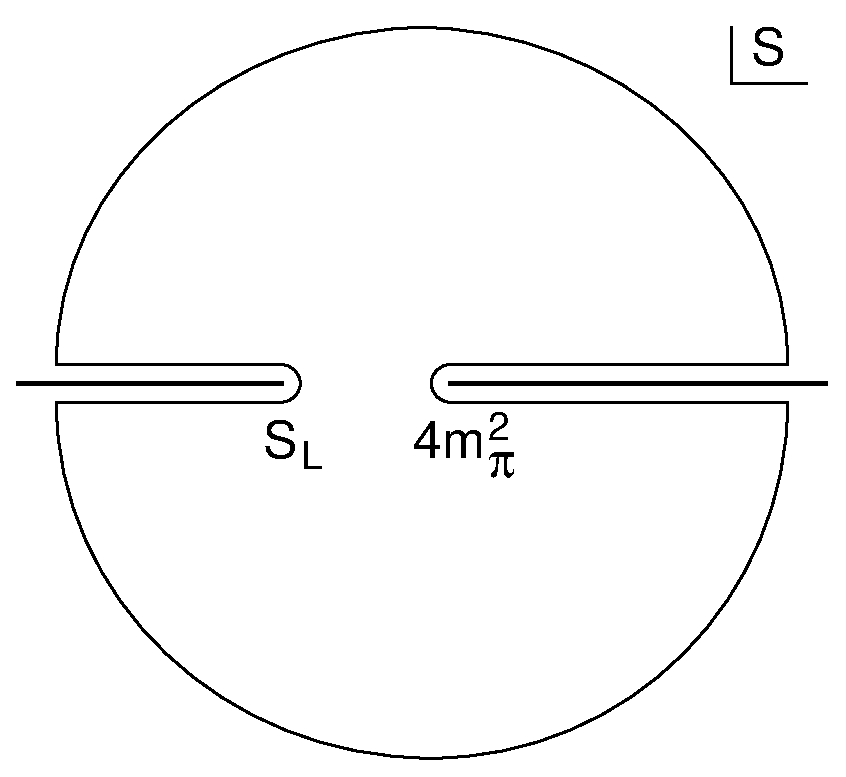
\psfig{file=ijcmf1.eps,width=5cm}}
\vspace*{8pt}
\caption{A schematic illustration of dissociative recombination. The
direct mechanism, 4m$^2_\pi$ is initiated when the molecular ion
S$_{\rm L}$ captures an electron with kinetic energy.\label{one}}
\end{figure}

Figure~\ref{one} are to be sequentially numbered in Arabic
numerals. The caption must be placed below the figure. Typeset in 8 pt  
roman with baselineskip of 10~pt. Long captions are to be justified by
the ``page-width''.  Use double spacing between a caption and the text
that follows immediately.

Previously published material must be accompanied by written
permission from the author and publisher.

\section{Tables}
Tables should be inserted in the text as close to the point of
reference as possible. Some space should be left above and below
the table.

Table~\ref{tab1} should be numbered sequentially in the text in Arabic
numerals. Captions are to be centralized above the tables.  Typeset
tables and captions in 8 pt roman with baselineskip of 10 pt. Long
captions are to be justified by the ``table-width''.

\begin{table}[th]
\tbl{Comparison of acoustic for frequencies for piston-cylinder 
problem.\label{tab1}}
{\begin{tabular}{@{}cccc@{}} \toprule
Piston mass & Analytical frequency & TRIA6-$S_1$ model &
\% Error \\
& (Rad/s) & (Rad/s) \\ \colrule
1.0\hphantom{00} & \hphantom{0}281.0 & \hphantom{0}280.81 & 0.07 \\
0.1\hphantom{00} & \hphantom{0}876.0 & \hphantom{0}875.74 & 0.03 \\
0.01\hphantom{0} & 2441.0 & 2441.0\hphantom{0} & 0.0\hphantom{0} \\
0.001 & 4130.0 & 4129.3\hphantom{0} & 0.16\\ \botrule
\end{tabular} }
\begin{tabnote}
Table notes
\end{tabnote}
\begin{tabfootnote}
\tabmark{a} Table footnote A\\
\tabmark{b} Table footnote B
\end{tabfootnote}
\end{table}

If tables need to extend over to a second page, the continuation of
the table should be preceded by a caption, e.g.~``{\it Table~1.}
$(${\it Continued}$)$''. Notes to tables are placed below the final
row of the table and should be flushleft.  Footnotes in tables
should be indicated by superscript lowercase letters and placed beneath
the table.

\section{Running Heads}
Please provide a shortened runninghead (not more than eight words) for
the title of your paper. This will appear on the top right-hand side
of your paper.

\section{Footnotes}
Footnotes should be numbered sequentially in superscript lowercase
roman letters.\footnote{Footnotes should be typeset in 8 pt roman at
the bottom of the page.}

\section*{Acknowledgments}
This section should come before the References. Funding information
may also be included here.

\appendix

\section{Appendices}

Appendices should be used only when absolutely necessary. They should
come after the References. If there is more than one appendix, number
them alphabetically. Number displayed equations occurring in the
Appendix in this way, e.g.~(\ref{a1}), (A.2), etc.
\begin{equation}
\mu(n, t) = \frac{\sum^\infty_{i=1} 1(d_i < t, 
N(d_i) = n)}{\int^t_{\sigma=0} 1(N(\sigma) = n)d\sigma}\,.
\label{a1}
\end{equation}

\section*{References}
The references section should be labeled ``References'' and should appear
at the end of the paper. Authors should follow a consistent format
for the reference entries. For journal names, use the standard abbreviations.
An sample format is given in the following page:

\subsection*{Citations in Text}
Since the references are unnumbered, citations to them in the text
must identify them by authors' names and year of
publication. References should be cited in text in square brackets by
giving the last name of the author and the date of publication,
e.g. \cite{wong89}. A comma should be present before the date.  For
papers by two authors, the last names are joined by ``and''
e.g. \cite{hussaini}. Papers by three and more authors should be cited 
by  giving the last name of the first author followed by {\it et al}. 
and the date (note that {\it et al}. is in italics and that a period
follows the abbreviation al.).

References are given in brackets unless the author's name is part
of the sentence, e.g. ``the a-model \cite{gupta97}''
but ``according to \citeauthor{gupta97} \shortcite{gupta97}.''
If a citation cites two or more papers, they should be separated 
by a semicolon: \cite{gurland94,wong89}. 
If two or more papers by the same author(s) are cited together, the 
author(s) should be listed once, with the dates of the papers separated
by a semicolon: 
(\citeauthor{gurland94}, \citeyear{gurland94}; \citeyear{gurland95}). 
Papers by the same author(s) published in the same 
year should be distinguished by appending a, b, c, etc., to the 
date: e.g. (\citeauthor{gupta95a}, \citeyear{gupta95a}; \citeyear{gupta95b}).

\subsection*{Reference List}
Reference entries should be ordered alphabetically, starting with the
last name of the first author, followed by the first author's
initial(s), and so on for each additional author. For papers with more
than three authors, the last name and initials of the first author
only should be listed, followed by a comma and {\it et al}.  Multiple 
entries for one author or one group of authors should be ordered
chronologically, and multiple entries for the same year (including
references with three authors that may be cited in the text as 
``{\it et al}.'') should be distinguished by appending sequential 
lowercase letters to the year; e.g. Gupta and Akman (1995a); 
Gupta and Akman (1995b).

\begin{thebibliography}
\bibitem[\protect\citeauthoryear{Al-Hussaini and 
Abd-El-Hakim}{1989}]{hussaini} 
Al-Hussaini, E. K. and Abd-El-Hakim, N. S. (1989). Failure rate of the 
inverse Gaussian-Weibull mixture model. {\it Ann. Inst. Stat. Math.}, 
{\bf 41}: 617--622.

\bibitem[\protect\citeauthoryear{Bradley and Gupta}{2001}]{braley} 
Bradley, D. M. and Gupta, R. C. (2001). The mean residual life and 
its limiting behaviour. Submitted for publication.

\bibitem[\protect\citeauthoryear{Chhikara and Folks}{1977}]{chhikara} 
Chhikara, R. S. and Folks, J. L. (1977). The inverse Gaussian 
distribution as a lifetime model. {\it Technometrics,} {\bf 19}: 
461--468.

\bibitem[\protect\citeauthoryear{Gupta and Akman}{1995a}]{gupta95a} 
Gupta, R. C. and Akman, O. (1995a). Mean residual life function 
for certain types of non-monotonic ageing. 
{\it Comm. Stat. Stoch. Models,} {\bf 11}, 3, pp.~219--225.

\bibitem[\protect\citeauthoryear{Gupta and Akman}{1995b}]{gupta95b} 
Gupta, R. C. and Akman, O (1995b). On the reliability studies of a 
weighted inverse Gaussian model. {\it J. Stat. Planning Inference}, 
{\bf 48}: 69--83.

\bibitem[\protect\citeauthoryear{Gupta {\it et~al}.}{1997}]{gupta97} 
Gupta, R. C., Kannan, N. and Raychaudhari, A. (1997). Analysis of 
log normal survival data. {\it Math. Biosci.}, {\bf 139}: 103--115.

\bibitem[\protect\citeauthoryear{Gurland and Sethuraman}{1994}]{gurland94} 
Gurland, J. and Sethuraman, J. (1994). Reversal of increasing 
failure rates when pooling failure data. {\it Technometrics,} 
{\bf 36}: 416--418.

\bibitem[\protect\citeauthoryear{Gurland and Sethuraman}{1995}]{gurland95} 
Gurland, J. and Sethuraman, J. (1995). How pooling data may 
reverse increasing failure rate. {\it J. Am. Stat. Assoc.}, 
{\bf 90}: 1416--1423.

\bibitem[\protect\citeauthoryear{Jorgensen {\it et~al}.}{1991}]{jorgensen} 
Jorgensen, B., Seshadri, V. and Whitmore, G. A. (1991). On the 
mixture of the inverse Gaussian distribution with its complementary 
reciprocal. {\it Scand. J. Stat.}, {\bf 18}: 77--89.

\bibitem[\protect\citeauthoryear{Mills}{1971}]{mills71} 
Mills, E. S. (1971). The value of urban land. {\it The 
Quality of the Urban Environment}, ed.~H. S. Perloff, Wiley, New York.

\bibitem[\protect\citeauthoryear{Park}{1999}]{park99} 
Park, W. R. (1999). {\it The Theory and Practice of
Econometrics}, 2nd edn. Wiley, New York.

\bibitem[\protect\citeauthoryear{Tang {\it et~al}.}{1999}]{tang} 
Tang, L. C., Lu, Y. and Chew, E. P. (1999). Mean residual lifetime 
distributions. {\it IEEE Trans. Reliabil.}, {\bf 48}: 73--78.

\bibitem[\protect\citeauthoryear{Winkler {\it et~al}.}{1972}]{winkler} 
Winkler, R. L., Roodman, G. M. and Britney, R. R. (1972). The 
determination of partial moments. {\it Manag. Sci.}, 
{\bf 19}: 290--296.

\bibitem[\protect\citeauthoryear{Wong}{1988}]{wong88} 
Wong, K. L. (1988). The bathtub does not hold water any more.  
{\it Qual. Reliabil. Eng. Int.}, {\bf 4}: 279--282.

\bibitem[\protect\citeauthoryear{Wong}{1989}]{wong89} 
Wong, K. L. (1989). The roller-coaster curve is in. 
{\it Qual. Reliabil. Eng. Int.}, {\bf 5}: 29--36.

\bibitem[\protect\citeauthoryear{Wong}{1991}]{wong91} 
Wong, K. L. (1991). The physical basis for the roller-coaster 
hazard rate curve for electronics. {\it Qual. Reliabil. 
Eng. Int.}, {\bf 7}: 489--495.
\end{thebibliography}

\end{document}



